\subsection{Regular diffusion}
The idea of diffusion is to fix the known regions of the image and let them diffuse into the unknown regions. This can be done very efficiently by using a convolutional kernel. By iteratively convolving a kernel with the entire image and then restoring the known pixels we can obtain an inpainted image. This process is described in algorithm \ref{alg:diffusion}. The quality of the solution heavily depends on the kernel used. A variety of kernels can be used, some of which are displayed in figure \ref{fig:kernels}.

\begin{figure}
\begin{flalign*}
K_{\text{diamond}} &= \begin{bmatrix}0 & 0.25 & 0 \\ 0.25 & 0 & 0.25 \\ 0 & 0.25 & 0\end{bmatrix}\\
K_{\text{gauss}} &= \begin{bmatrix}0.011 & 0.084 & 0.011\\0.084 & 0.620 & 0.084 \\0.011 & 0.084 & 0.011\end{bmatrix}\\
K_{\text{diag}} &= \begin{bmatrix}0.38 & 0.04 & 0.04 \\ 0.04 & 0 & 0.04 \\ 0.04 & 0.04 & 0.38\end{bmatrix}
\end{flalign*}
\caption{Kernels used for diffusion.}
\label{fig:kernels}
\end{figure}

\begin{algorithm}
	\KwIn{Image $I$, mask $M$, kernel $K$ and threshold $\epsilon$}
	\KwResult{Reconstructed image $I_{r}$}
	$K \leftarrow \frac{1}{\sum_i \sum_j K_{i,j}} * K$\;
	$I_{prev} \leftarrow 0_{size(I)}$\;
	$I_{r} \leftarrow I$\;
	\While{$\|I_{r} - I_{prev} \|_{F} > \epsilon$}{
		$I_{prev} \leftarrow I_{r}$\;
		$I_{r} \leftarrow \text{convolve}(I_{r}, K)$\;
		$I_{r} \leftarrow I_{r} \circ \mathrm{I}_{M = 0} + I \circ \mathrm{I}_{M \neq 0}$ \;
	}
	\quad
\caption{Diffusion algorithm for inpainting.}
\label{alg:diffusion}
\end{algorithm}

\begin{figure}
	\centering
	\begin{subfigure}[b]{0.45\textwidth}
		\centering
		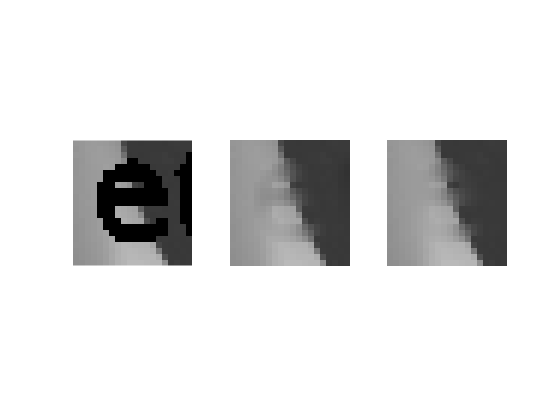
\includegraphics[clip, trim=0cm 1cm 0cm 0.5cm, width=0.85\textwidth]{figures/step-by-step-cross}
		\caption{Diamond kernel $K_{diamond}$}
		\label{fig:stepbystepcross}
	\end{subfigure}
	\begin{subfigure}[b]{0.45\textwidth}
		\centering
		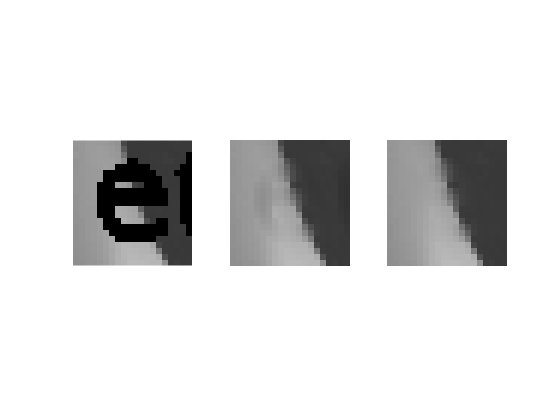
\includegraphics[clip, trim=0cm 1cm 0cm 0.5cm, width=0.85\textwidth]{figures/step-by-step-directional}
		\caption{Directional kernel $K_\theta$ for $\theta = 146$.}
		\label{fig:stepbystepdir}
	\end{subfigure}
	\caption{Step-by-step illustration of the diffusion process with different kernels. Each step represent 20 iterations.}
\end{figure}